
%(BEGIN_QUESTION)
% Copyright 2006, Tony R. Kuphaldt, released under the Creative Commons Attribution License (v 1.0)
% This means you may do almost anything with this work of mine, so long as you give me proper credit

A collection of operational amplifiers may be used to implement the following equation for a proportional controller, with each variable represented by a DC voltage:

$$m = K_p (\hbox{SP} - \hbox{PV}) + b$$

\noindent
Where,

$m$ = Manipulated variable (output)

$K_p$ = Controller gain

SP = Setpoint

PV = Process variable

$b$ = Bias

\vskip 10pt

$$\includegraphics[width=15.5cm]{i01465x01.eps}$$

Identify which module or modules implement each portion of the proportional control equation.

\medskip 
\item{}Module 1:
\vskip 5pt
\item{}Module 2:
\vskip 5pt
\item{}Module 3:
\vskip 5pt
\item{}Module 4:
\vskip 5pt
\item{}Module 5:
\vskip 5pt
\item{}Module 6:
\end{itemize} 

Also, identify whether this is a {\it direct-acting} or a {\it reverse-acting} controller.
 
\vskip 20pt \vbox{\hrule \hbox{\strut \vrule{} {\bf Suggestions for Socratic discussion} \vrule} \hrule}

\begin{itemize}
\item{} Demonstrate how you may apply the problem-solving technique of using a {\it thought experiment} to determine whether this controller is direct or reverse acting.
\item{} Randomly choose any one resistor in this controller circuit and imagine that resistor failing either {\it open} or {\it shorted}.  Then, explain the effects of that fault on the output signal of the controller.
\end{itemize}

\underbar{file i01465}
%(END_QUESTION)





%(BEGIN_ANSWER)

\medskip 
\item{}Module 1: Voltage follower (buffer) for PV signal
\vskip 5pt
\item{}Module 2: Voltage follower (buffer) for SP signal
\vskip 5pt
\item{}Module 3: Differential amplifier (calculates error signal)
\vskip 5pt
\item{}Module 4: Variable-gain amplifier (multiplies error signal by $K_p$, set by potentiometer)
\vskip 5pt
\item{}Module 5: Voltage follower (buffer) for bias signal
\vskip 5pt
\item{}Module 6: Summer, adds bias signal to output of amplifier
\end{itemize} 
 
\vskip 10pt

This is a {\it reverse-acting} controller.

%(END_ANSWER)





%(BEGIN_NOTES)


%INDEX% Control, proportional: analog electronic controller

%(END_NOTES)


